\begin{figure*}[t]
\centering
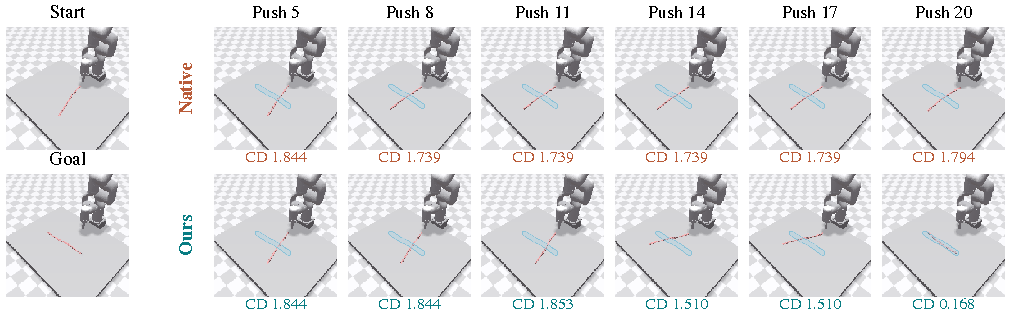
\includegraphics[width=0.90\textwidth]{figures/fig_rope_main_rollout.pdf}
\caption{\textbf{Rope recovery at matched push counts.} DINO-WM runs share the start and goal; Ours adds fixed-strength ECP after five warm-up pushes. Pale blue marks the goal rope; labels give Chamfer distance (CD). Only ECP reaches CD $<0.3$ at push 20.}
\label{fig:rope-main-rollout}
\par\vspace{2pt}
\begin{minipage}[t]{0.485\textwidth}\vspace{0pt}
\centering
\captionof{table}{\textbf{ECP improves Rope planning.} Fixed DINO-WM, three pushes per plan. Ours adds fixed-strength memory after five warm-up pushes. Twenty targets repeat under three seeds (60 runs). CD is mean final Chamfer distance; success requires CD $<0.3$. Pushes averages all runs, including failures capped at 20.}
\label{tab:rope}
\small
\begin{tabular*}{\linewidth}{@{\extracolsep{\fill}}lrrr@{}}
\toprule
Method & CD $\downarrow$ & Success (\%) $\uparrow$ & Pushes $\downarrow$\\
\midrule
DINO-WM (native) &0.6865&55.0&12.68\\
DINO-WM (ours) &\textbf{0.4793}&\textbf{71.7}&\textbf{11.30}\\
\bottomrule
\end{tabular*}
\end{minipage}
\hfill
\begin{minipage}[t]{0.485\textwidth}\vspace{0pt}
\centering
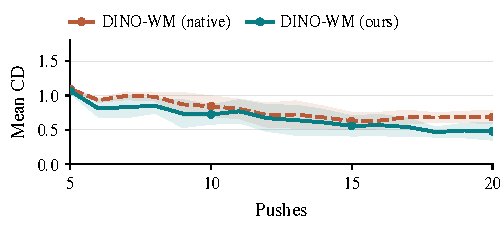
\includegraphics[width=\linewidth]{figures/fig_rope_cd_pushes.pdf}
\captionof{figure}{\textbf{Faster Rope error reduction.} DINO-WM with three pushes per plan; 20 targets under three seeds. Ours uses fixed-strength memory with five warm-up pushes.}
\label{fig:rope-cd}
\end{minipage}
\end{figure*}
